\documentclass[12pt,]{article}
%\usepackage{lmodern}  Melissa removed to deal with font rendering issue
\usepackage{amssymb,amsmath}
\usepackage{ifxetex,ifluatex}
\usepackage{fixltx2e} % provides \textsubscript

%Melissa removed the following section to deal with font rendering issue
%\ifnum 0\ifxetex 1\fi\ifluatex 1\fi=0 % if pdftex
%  \usepackage[T1]{fontenc}
%  \usepackage[utf8]{inputenc}
%%\else % if luatex or xelatex
%  \ifxetex
%    \usepackage{mathspec}
%  \else
%    \usepackage{fontspec}
%  \fi
%  \defaultfontfeatures{Ligatures=TeX,Scale=MatchLowercase}
%  \newcommand{\euro}{€}
%%%%%%\fi

% use upquote if available, for straight quotes in verbatim environments
\IfFileExists{upquote.sty}{\usepackage{upquote}}{}
% use microtype if available
\IfFileExists{microtype.sty}{%
\usepackage{microtype}
\UseMicrotypeSet[protrusion]{basicmath} % disable protrusion for tt fonts
}{}
\usepackage[margin=1in]{geometry}
\usepackage{hyperref}
\PassOptionsToPackage{usenames,dvipsnames}{color} % color is loaded by hyperref
\hypersetup{unicode=true,
            pdftitle={Status of Gopher Rockfish (Sebastes carnatus) and Black-and-Yellow Rockfish (Sebastes chrysomelas) Off the California Coast in 2019},
            pdfborder={0 0 0},
            breaklinks=true}
\urlstyle{same}  % don't use monospace font for urls
\usepackage{graphicx,grffile}
\makeatletter
\def\maxwidth{\ifdim\Gin@nat@width>\linewidth\linewidth\else\Gin@nat@width\fi}
\def\maxheight{\ifdim\Gin@nat@height>\textheight\textheight\else\Gin@nat@height\fi}
\makeatother
% Scale images if necessary, so that they will not overflow the page
% margins by default, and it is still possible to overwrite the defaults
% using explicit options in \includegraphics[width, height, ...]{}
\setkeys{Gin}{width=\maxwidth,height=\maxheight,keepaspectratio}
\setlength{\parindent}{0pt}
\setlength{\parskip}{6pt plus 2pt minus 1pt}
\setlength{\emergencystretch}{3em}  % prevent overfull lines
\providecommand{\tightlist}{%
  \setlength{\itemsep}{0pt}\setlength{\parskip}{0pt}}
\setcounter{secnumdepth}{5}

%%% Use protect on footnotes to avoid problems with footnotes in titles
\let\rmarkdownfootnote\footnote%
\def\footnote{\protect\rmarkdownfootnote}

%%% Change title format to be more compact
\usepackage{titling}

% Create subtitle command for use in maketitle
\newcommand{\subtitle}[1]{
  \posttitle{
    \begin{center}\large#1\end{center}
    }
}

\setlength{\droptitle}{-2em}
  \title{Status of Gopher Rockfish (\emph{Sebastes carnatus}) and
Black-and-Yellow Rockfish (\emph{Sebastes chrysomelas}) Off the
California Coast in 2019}
  \pretitle{\vspace{\droptitle}\centering\huge}
  \posttitle{\par}
  \author{}
  \preauthor{}\postauthor{}
  \date{}
  \predate{}\postdate{}


% This file contains all of the LaTeX packages you may need to compile the document
% Documentation for each package can be found onlines
\usepackage{tabularx}                                             % table environment providing flexibility
\usepackage{caption}                                              % for creating captions  
\usepackage{longtable}                                            % allows tables to span multiple pages
\usepackage{rotating}                                             % allows for sideways tables
\usepackage{float}                                                % floating environments; may not need in rmarkdown
\usepackage{placeins}                                             % keeps floats from moving
\usepackage{indentfirst}                                          % indents first paragraph of a section
\usepackage{mdwtab}                                               % continued float multi-page figure
\usepackage{enumerate}                                            % create lists
\usepackage{hyperref}                                             % highlight cross references
\hypersetup{colorlinks=true, urlcolor=blue, linktoc=page, linkcolor=blue, citecolor=blue} %define referencing colors
%\usepackage{makebox}                                             % make boxes around text
\usepackage[usenames,dvipsnames]{xcolor}                          % color name options
%\usepackage[space]{grffile}                                      % spaces in file name path
\usepackage{soul}                                                 % highlight text
\usepackage{enumitem}                                             % numbered lists
\usepackage{lineno}                                               % Line numbers; comment out for final
\usepackage{upquote}                                              % produce grave accent in latex
\usepackage{verbatim}                                             % produces verbatim results
\usepackage{fancyvrb}                                             % verbatim in a box
%\usepackage{draftwatermark}                                      % places Draft watermark in background; comment out for final
\usepackage{textcomp}                                             % fixes error with packages interfering
\usepackage{lscape}                                               % rotate pages - to allow for landscape longtables
%\pdfinterwordspaceon                                             % fix loss of inter word spacing
\usepackage{cmap}                                                 % fix mapping characters to unicode
\RequirePackage[linewidth = 1]{pdfcomment}                        % pdf comments
\RequirePackage[l2tabu, orthodox]{nag}                            % checks packages related to the accessibility?
\usepackage[inline]{showlabels}                                   % show table and figure labels; comment out for final
%\RequirePackage[tagged]{accessibilityMeta}


\linenumbers                                                      % specify use of line numbers


\definecolor{light-gray}{gray}{.85}                               % define light-gray as a color
%\usepackage[tagged]{accessibility-meta}

 
%\showlabels[\color{mred}]{label}

% Redefines (sub)paragraphs to behave more like sections
\ifx\paragraph\undefined\else
\let\oldparagraph\paragraph
\renewcommand{\paragraph}[1]{\oldparagraph{#1}\mbox{}}
\fi
\ifx\subparagraph\undefined\else
\let\oldsubparagraph\subparagraph
\renewcommand{\subparagraph}[1]{\oldsubparagraph{#1}\mbox{}}
\fi

\begin{document}
\maketitle


\begin{center}
\thispagestyle{empty}


\vspace{.5cm}

%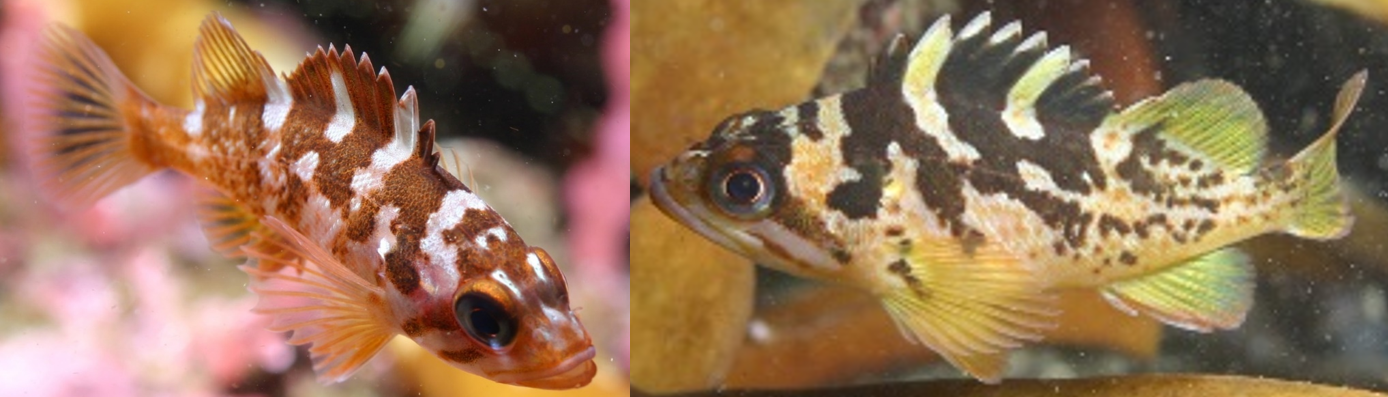
\includegraphics{cover_photo}~\\[1cm]
\pdftooltip{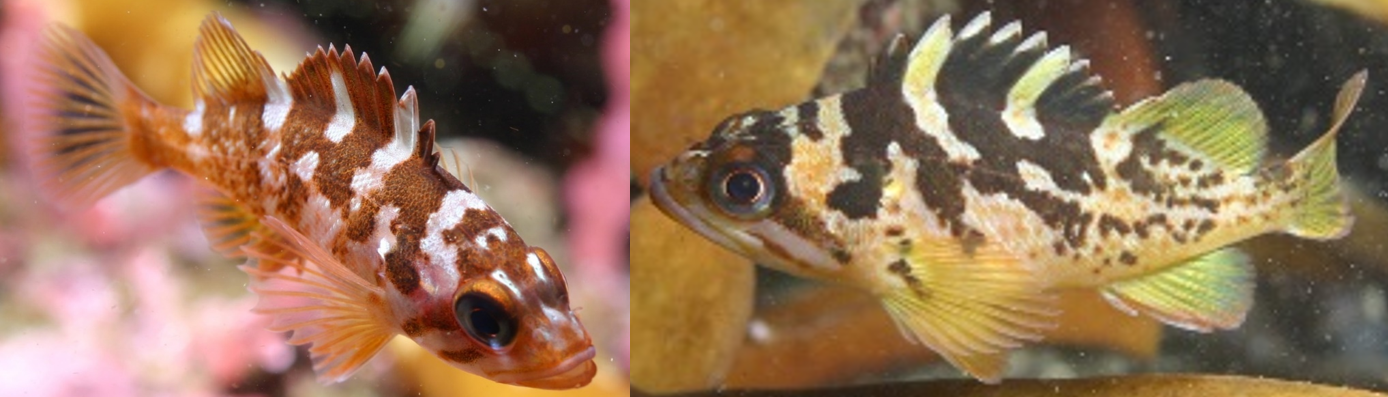
\includegraphics{cover_photo}}{This is a fish.}
Gopher rockfish (left) and black-and-yellow rockfish (right).      
\small
Photos courtsey Steve Lonhart.

\vspace{.3cm}


Melissa H. Monk\textsuperscript{1}\\
Xi He\textsuperscript{1}\\

\vspace{.5cm}

\small
\textsuperscript{1}Southwest Fisheries Science Center, U.S. Department of Commerce, National Oceanic and Atmospheric Administration, National Marine Fisheries Service, 110 McAllister Way, Santa Cruz, California 95060\\

\vspace{1.5cm}


%\vfill
DRAFT SAFE\\
Disclaimer: This information is distributed solely for the purpose of pre-dissemination
peer review under applicable information quality guidelines. It has not been formally
disseminated by NOAA Fisheries. It does not represent and should not be construed to
represent any agency determination or policy. 

\vspace{.1cm}
%Bottom of the page
{\large \today}


\newpage{\thispagestyle{empty}}


\begin{flushleft}

\end{flushleft}

\maketitle

\pagenumbering{roman}
\setcounter{page}{1}
\end{center}

{
\setcounter{tocdepth}{4}
\tableofcontents
}
\setlength{\parskip}{5mm plus1mm minus1mm} \pagebreak

\setcounter{page}{1} \renewcommand{\thefigure}{\alph{figure}}
\renewcommand{\thetable}{\alph{table}}

\section*{Executive Summary}\label{executive-summary}
\addcontentsline{toc}{section}{Executive Summary}

\subsection*{Stock}\label{stock}
\addcontentsline{toc}{subsection}{Stock}

This assessment reports the status of the GBY rockfish
(\emph{Sebastes carnatus/Sebastes chrysomelas}) resource in U.S. waters
off the coast of \ldots{} using data through 2018.

\subsection*{Catches}\label{catches}
\addcontentsline{toc}{subsection}{Catches}

Information on historical landings of GBY rockfish are available back to
xxxx\ldots{} (Table \ref{tab:Exec_catch}). Commercial landings were
small during the years of World War II, ranging between 4 to 27 metric
tons (mt) per year.

(Figures \ref{fig:Exec_catch1}-\ref{fig:Exec_catch2})\\
(Figure \ref{fig:r4ss_catches})

Since 2000, annual total landings of GBY rockfish have ranged between
69-159 mt, with landings in 2018 totaling 93 mt.

\FloatBarrier

\begin{figure}
\centering
\includegraphics{00_Assessment_Compile_files/figure-latex/unnamed-chunk-3-1.pdf}
\caption{GBY rockfish catch history for the recreational fleets.
\label{fig:Exec_catch1}}
\end{figure}

\begin{figure}
\centering
\includegraphics{00_Assessment_Compile_files/figure-latex/unnamed-chunk-4-1.pdf}
\caption{Stacked line plot of GBY rockfish catch history for the
commercial fleets. \label{fig:Exec_catch2}}
\end{figure}

\FloatBarrier

\begin{figure}
\centering
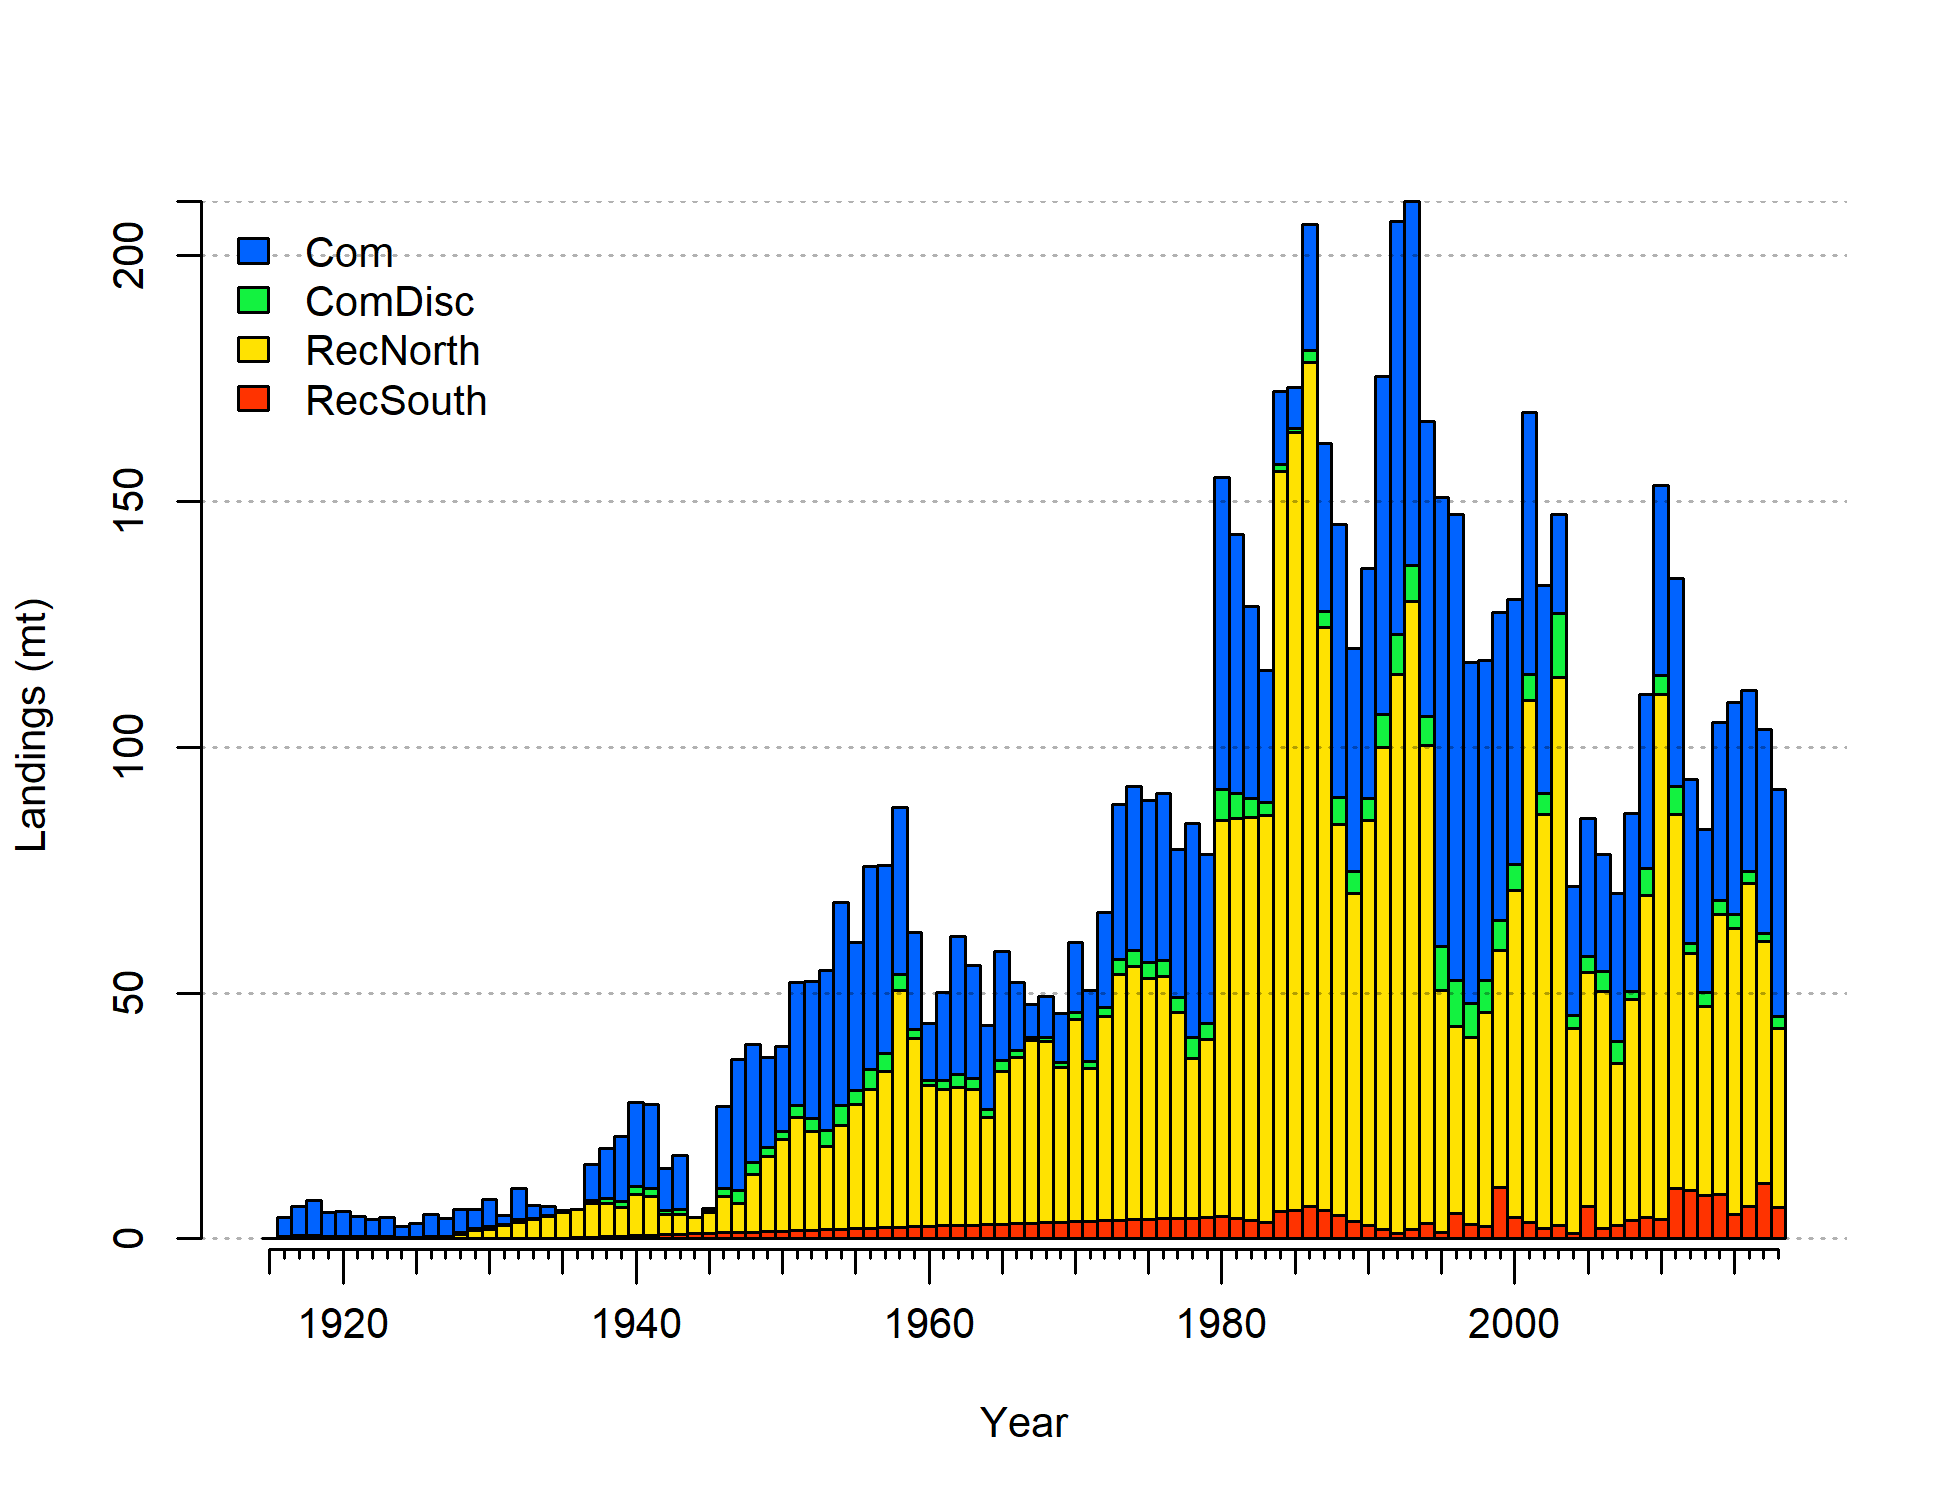
\includegraphics{r4ss/plots_mod1/catch2 landings stacked.png}
\caption{Catch history of GBY rockfish in the model.
\label{fig:r4ss_catches}}
\end{figure}

\begin{table}[ht]
\centering
\caption{Recent GBY rockfish landings (mt) by 
                                            fleet.} 
\label{tab:Exec_catch}
\begin{tabular}{l>{\centering}p{1in}>{\centering}p{1in}>{\centering}p{1in}>{\centering}p{.9in}>{\centering}p{.9in}>{\centering}p{.6in}}
  \hline
Year & Landings 1 & Landings 2 & Landings 3 & Landings 4 & Landings 5 & Total \\ 
  \hline
2005 & - & - & - & - & - & - \\ 
  2006 & - & - & - & - & - & - \\ 
  2007 & - & - & - & - & - & - \\ 
  2008 & - & - & - & - & - & - \\ 
  2009 & - & - & - & - & - & - \\ 
  2010 & - & - & - & - & - & - \\ 
  2011 & - & - & - & - & - & - \\ 
  2012 & - & - & - & - & - & - \\ 
  2013 & - & - & - & - & - & - \\ 
  2014 & - & - & - & - & - & - \\ 
   \hline
\end{tabular}
\end{table}

\FloatBarrier

\newpage

\subsection*{Data and Assessment}\label{data-and-assessment}
\addcontentsline{toc}{subsection}{Data and Assessment}

This a new full assessment for GBY rockfish, which was last assessed in
\ldots{} using Stock Synthesis Version xx. This assessment uses the
newest version of Stock Synthesis (3.30.xx). The model begins in 1916,
and assumes the stock was at an unfished equilibrium that year.

(Figure \ref{fig:assess_region_map}).

\begin{figure}
\centering
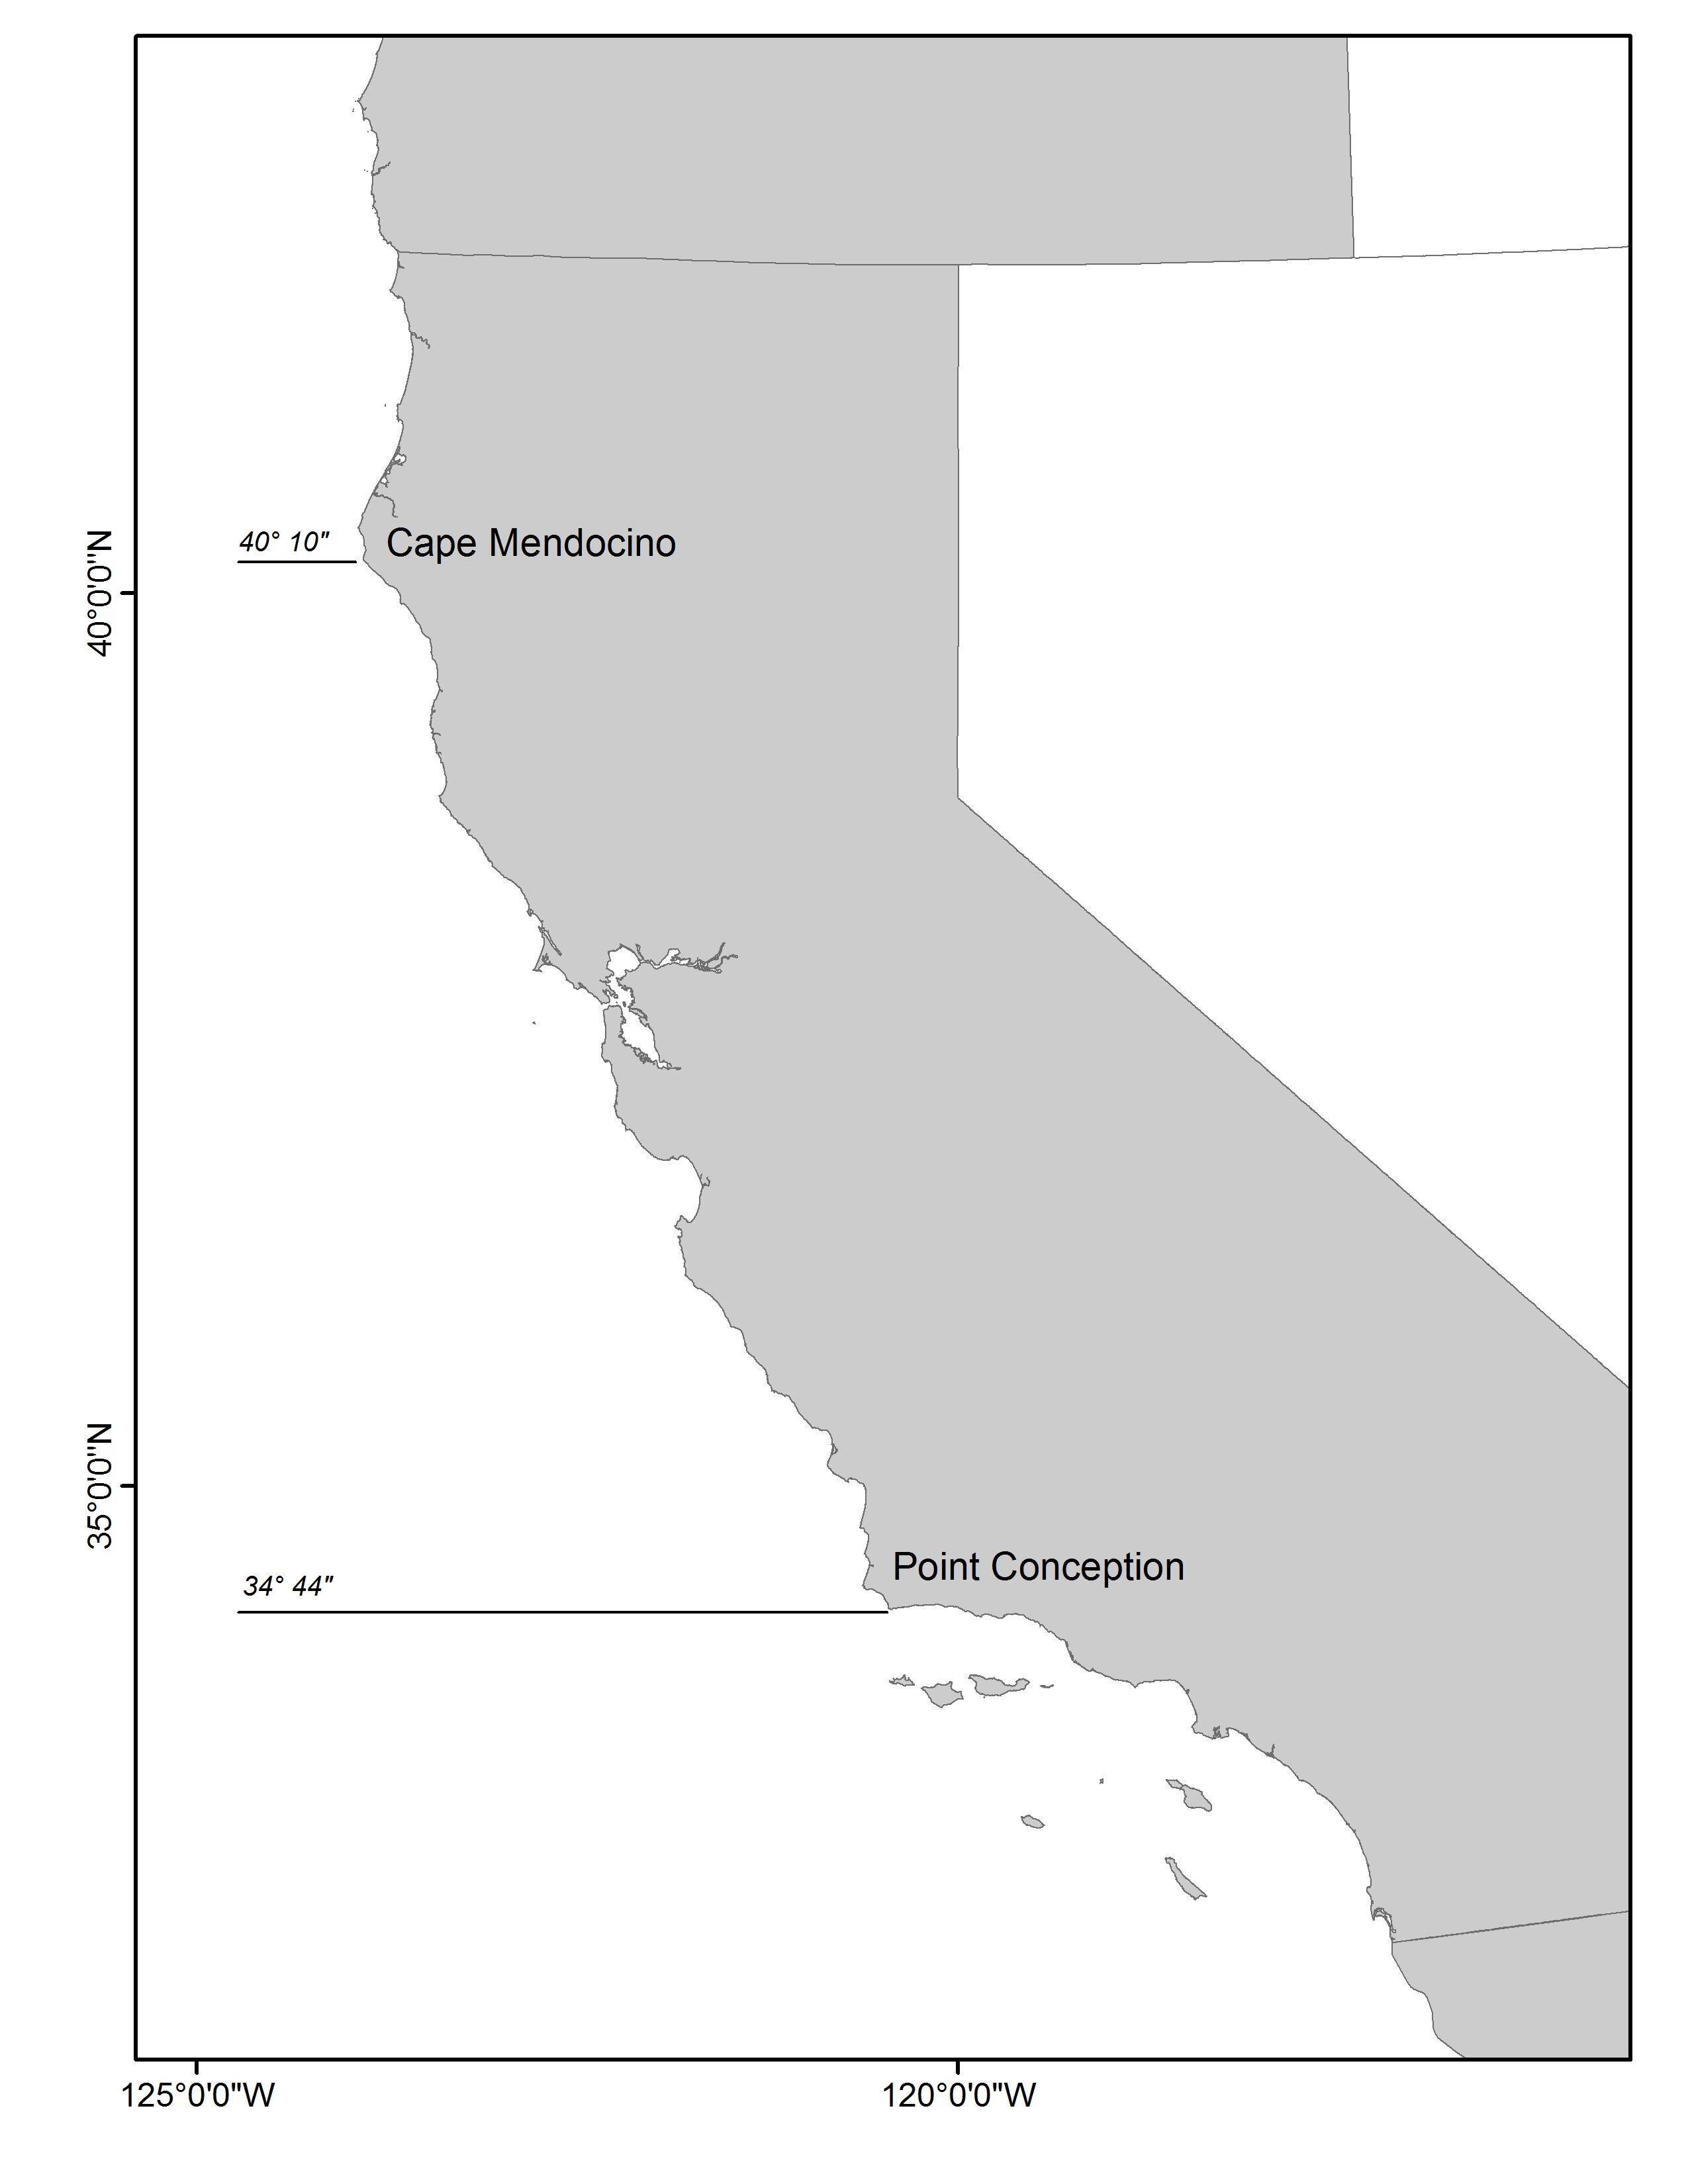
\includegraphics{Figures/assess_region_map.png}
\caption{Map depicting the distribution of California scorpionfish out
to 600 ft. The stock assessment is bounded at Pt. Conception in the
north to the U.S./Mexico border in the south.
\label{fig:assess_region_map}}
\end{figure}

\FloatBarrier

\subsection*{Stock Biomass}\label{stock-biomass}
\addcontentsline{toc}{subsection}{Stock Biomass}

(Figure \ref{fig:Spawnbio_all} and Table
\ref{tab:SpawningDeplete_mod1}).

The 2018 estimated spawning biomass relative to unfished equilibrium
spawning biomass is above the target of 40\% of unfished spawning
biomass at 45.1\% (95\% asymptotic interval: \(\pm\) 28.9\%-61.3\%)
(Figure \ref{fig:RelDeplete_all}). Approximate confidence intervals
based on the asymptotic variance estimates show that the uncertainty in
the estimated spawning biomass is high.

\FloatBarrier

\begin{table}[ht]
\centering
\caption{Recent trend in beginning of the 
                                      year spawning output and depletion for
                                      the model for GBY rockfish.} 
\label{tab:SpawningDeplete_mod1}
\begin{tabular}{l>{\centering}p{1.3in}>{\centering}p{1.2in}>{\centering}p{1in}>{\centering}p{1.2in}}
  \hline
Year & Spawning Output (million eggs) & \~{} 95\% confidence interval & Estimated depletion & \~{} 95\% confidence interval \\ 
  \hline
2010 & 864.575 & (604.3-1124.85) & 0.650 & (0.515-0.786) \\ 
  2011 & 795.859 & (549.68-1042.04) & 0.599 & (0.471-0.726) \\ 
  2012 & 741.221 & (507.57-974.88) & 0.558 & (0.437-0.678) \\ 
  2013 & 711.779 & (487.79-935.76) & 0.535 & (0.421-0.65) \\ 
  2014 & 691.107 & (474.44-907.77) & 0.520 & (0.41-0.63) \\ 
  2015 & 661.019 & (449.78-872.25) & 0.497 & (0.39-0.604) \\ 
  2016 & 634.707 & (425.9-843.51) & 0.477 & (0.371-0.584) \\ 
  2017 & 612.729 & (404.15-821.3) & 0.461 & (0.353-0.569) \\ 
  2018 & 599.056 & (389.03-809.08) & 0.451 & (0.34-0.561) \\ 
  2019 & 599.431 & (397.31-801.55) & 0.451 & (0.289-0.613) \\ 
   \hline
\end{tabular}
\end{table}

\FloatBarrier

\begin{figure}
\centering
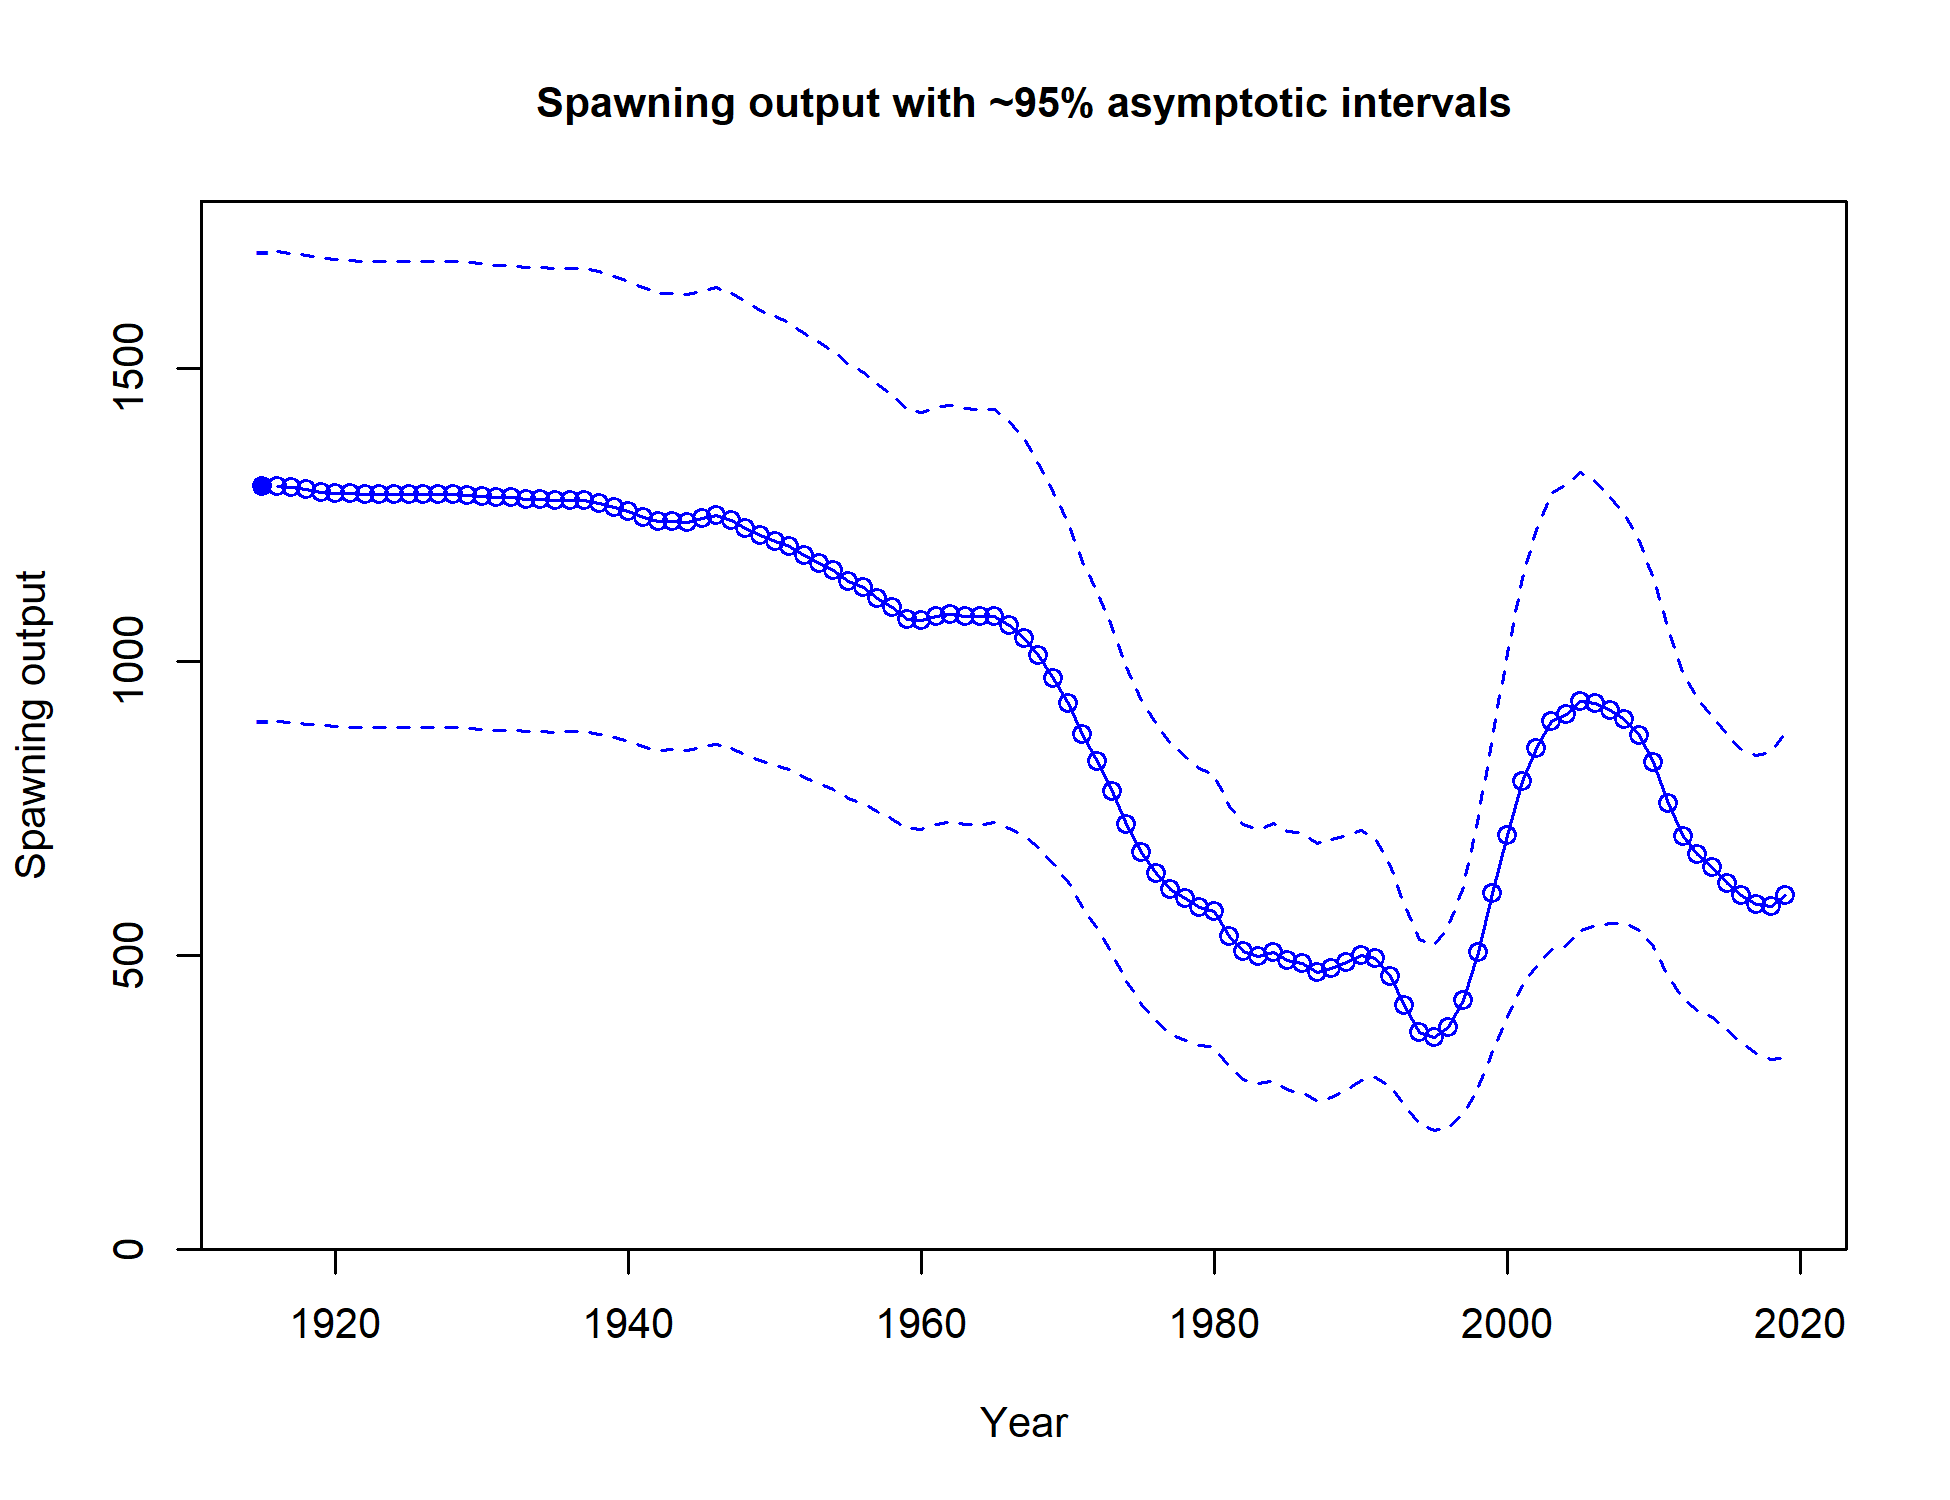
\includegraphics{r4ss/plots_mod1/ts7_Spawning_output_with_95_asymptotic_intervals_intervals.png}
\caption{Time series of spawning biomass trajectory (circles and line:
median; light broken lines: 95\% credibility intervals) for the base
case assessment model. \label{fig:Spawnbio_all}}
\end{figure}

\begin{figure}
\centering
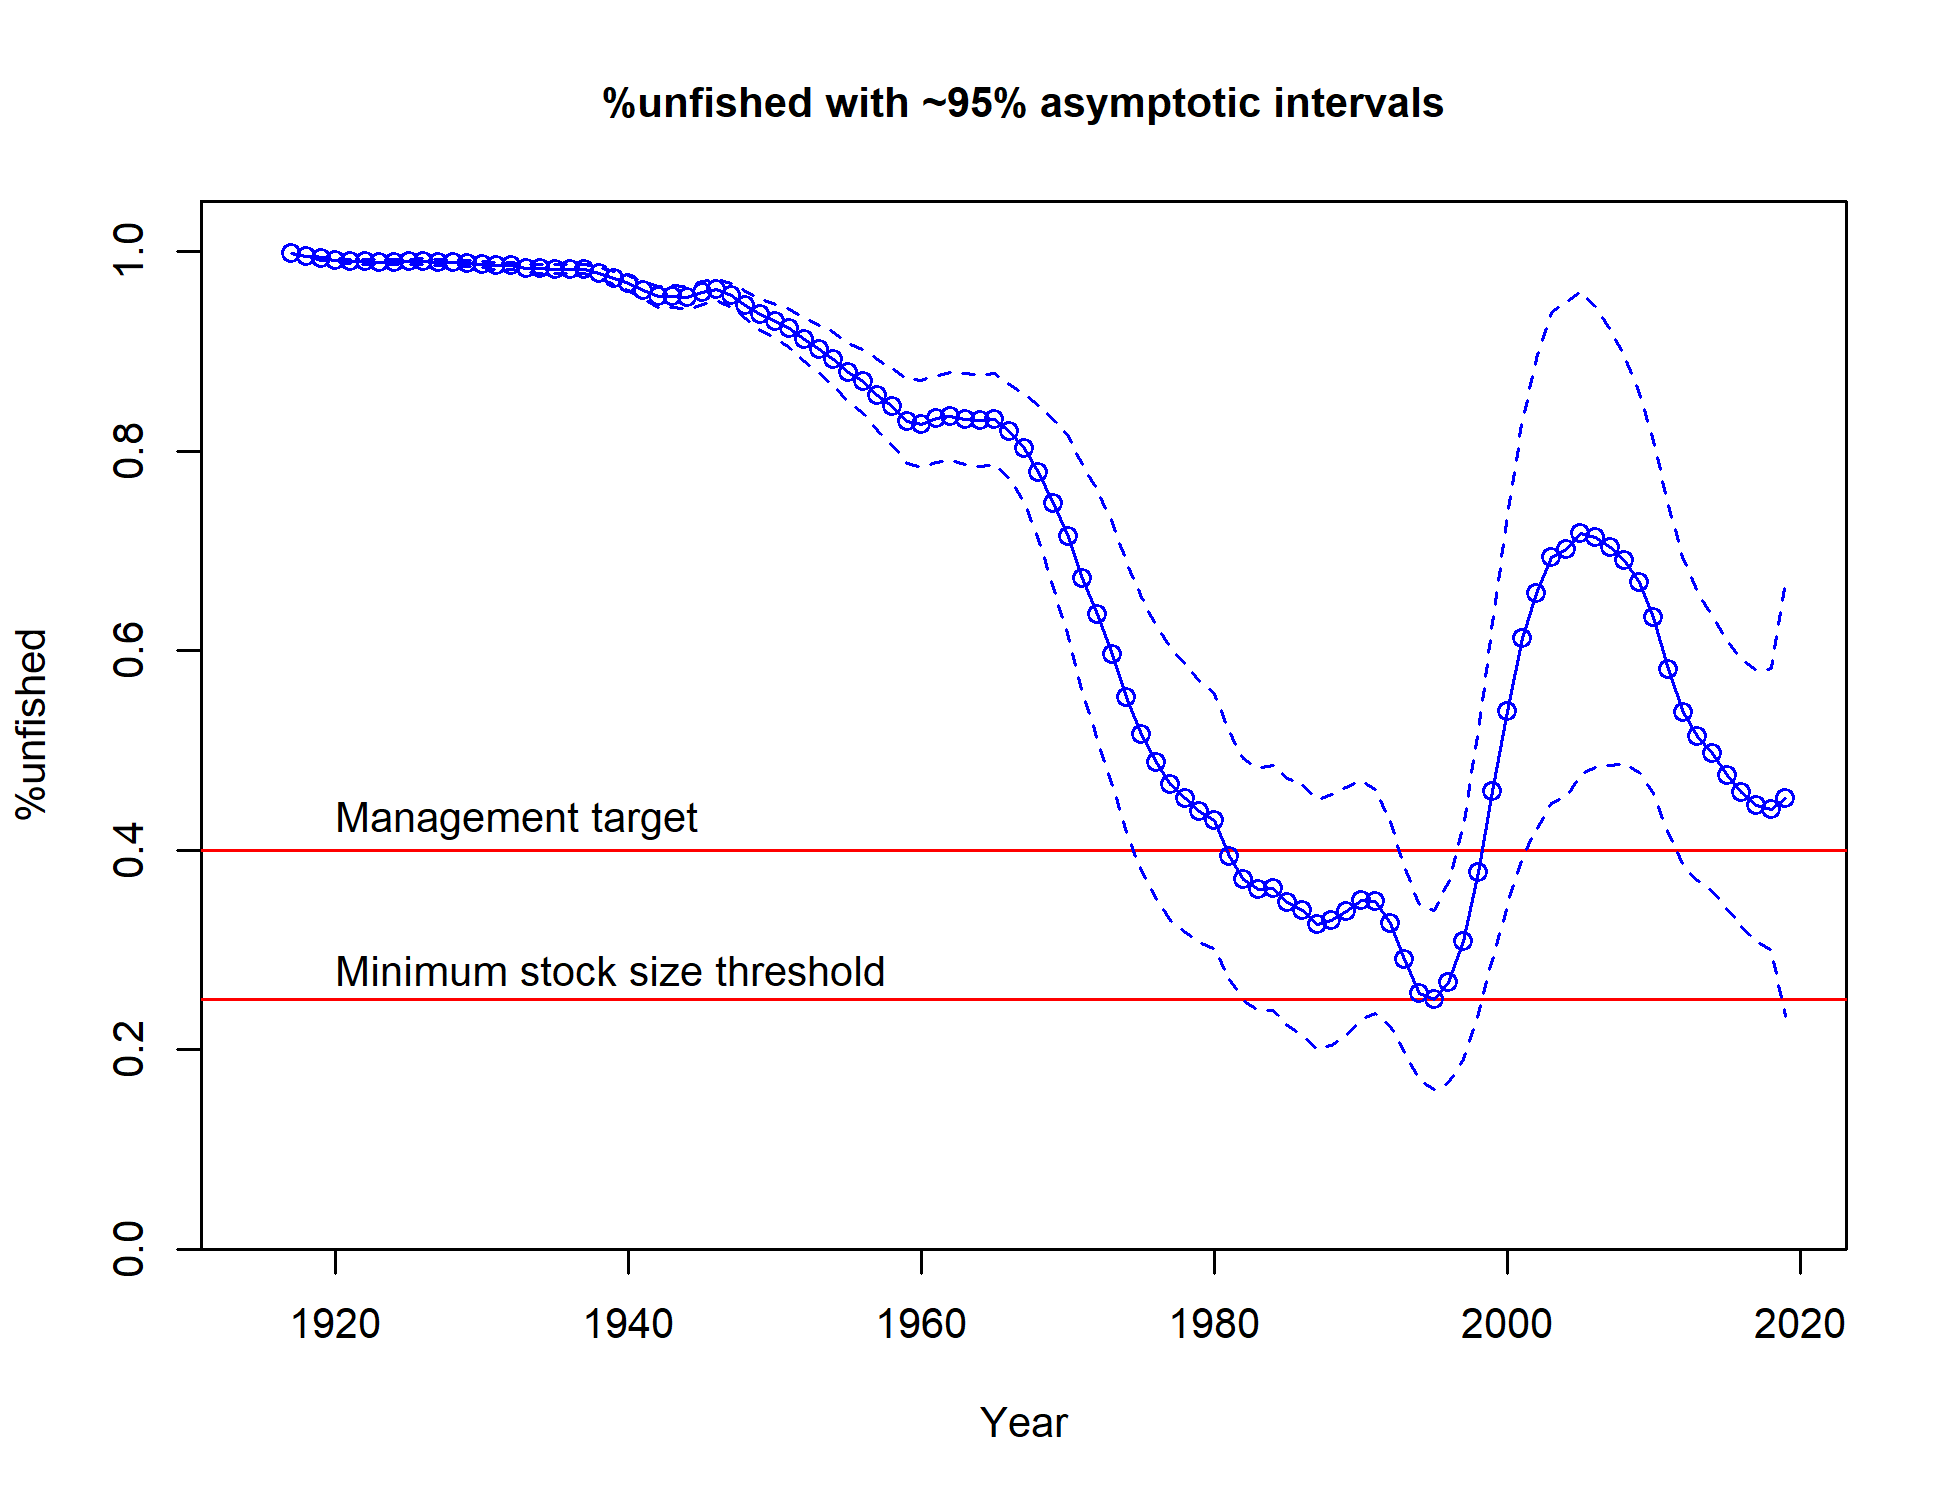
\includegraphics{r4ss/plots_mod1/ts9_unfished_with_95_asymptotic_intervals_intervals.png}
\caption{Estimated percent depletion with approximate 95\% asymptotic
confidence intervals (dashed lines) for the base case assessment model.
\label{fig:RelDeplete_all}}
\end{figure}

\FloatBarrier

\subsection*{Recruitment}\label{recruitment}
\addcontentsline{toc}{subsection}{Recruitment}

Recruitment deviations were estimated from xxxx-xxxx (Figure
\ref{fig:Recruits_all} and Table \ref{tab:Recruit_mod1}).

\begin{table}[ht]
\centering
\caption{Recent recruitment for the model.} 
\label{tab:Recruit_mod1}
\begin{tabular}{>{\centering}p{.8in}>{\centering}p{1.6in}>{\centering}p{1.3in}}
  \hline
Year & Estimated Recruitment (1,000s) & \~{} 95\% confidence interval \\ 
  \hline
2010 & 3218.83 & (1410.42 - 7345.97) \\ 
  2011 & 2746.99 & (1180.57 - 6391.77) \\ 
  2012 & 2631.66 & (1126.64 - 6147.16) \\ 
  2013 & 2767.28 & (1179.6 - 6491.88) \\ 
  2014 & 3916.77 & (1632.26 - 9398.66) \\ 
  2015 & 5510.34 & (2305.44 - 13170.55) \\ 
  2016 & 4079.14 & (1645.01 - 10115.07) \\ 
  2017 & 3360.32 & (1372 - 8230.16) \\ 
  2018 & 2968.86 & (1262.36 - 6982.25) \\ 
  2019 & 3352.25 & (1373.02 - 8184.58) \\ 
   \hline
\end{tabular}
\end{table}

\FloatBarrier

\begin{figure}
\centering
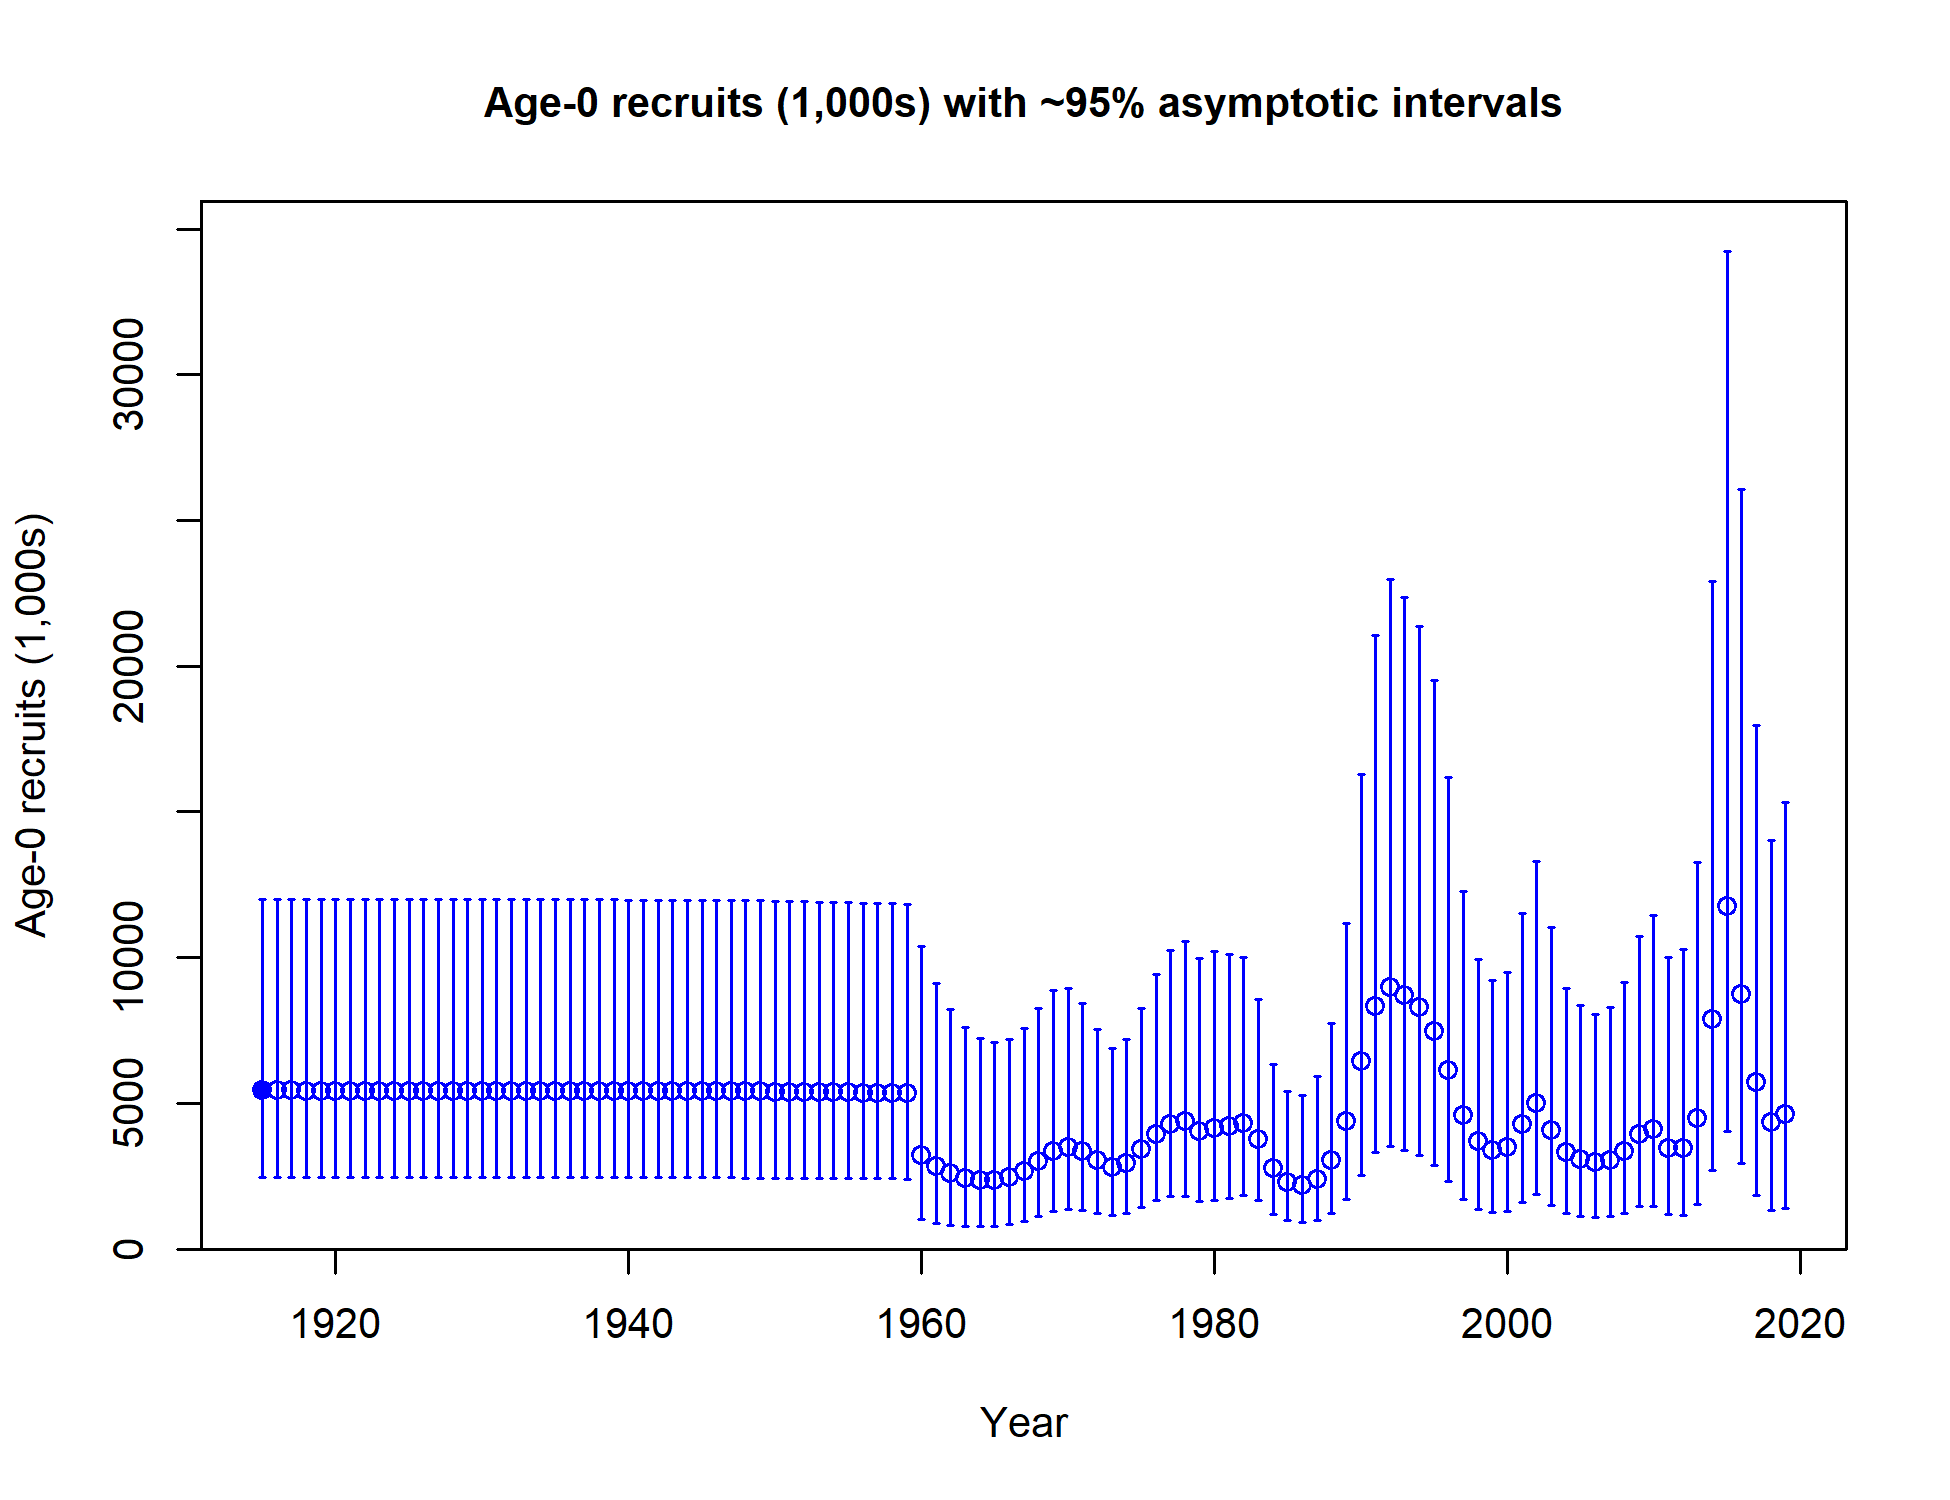
\includegraphics{r4ss/plots_mod1/ts11_Age-0_recruits_(1000s)_with_95_asymptotic_intervals.png}
\caption{Time series of estimated GBY rockfish recruitments for the
base-case model with 95\% confidence or credibility intervals.
\label{fig:Recruits_all}}
\end{figure}

\FloatBarrier

\subsection*{Exploitation status}\label{exploitation-status}
\addcontentsline{toc}{subsection}{Exploitation status}

Harvest rates estimated by the base model \ldots{}.. management target
levels (Table \ref{tab:SPR_Exploit_mod1} and Figure \ref{fig:SPR_all}).

\FloatBarrier

\begin{table}[ht]
\centering
\caption{Recent trend in spawning potential 
                                        ratio and exploitation for GBY rockfish in the model.  Fishing intensity is (1-SPR) 
                                        divided by 50\% (the SPR target) and exploitation 
                                        is F divided by F\textsubscript{SPR}.} 
\label{tab:SPR_Exploit_mod1}
\begin{tabular}{l>{\centering}p{1in}>{\centering}p{1.2in}>{\centering}p{1in}>{\centering}p{1.2in}}
  \hline
Year & Fishing intensity & \~{} 95\% confidence interval & Exploitation rate & \~{} 95\% confidence interval \\ 
  \hline
2009 & 0.67 & (0.49-0.85) & 0.08 & (0.06-0.1) \\ 
  2010 & 0.82 & (0.63-1.02) & 0.11 & (0.08-0.15) \\ 
  2011 & 0.81 & (0.61-1.01) & 0.11 & (0.08-0.14) \\ 
  2012 & 0.71 & (0.52-0.9) & 0.08 & (0.06-0.1) \\ 
  2013 & 0.67 & (0.49-0.86) & 0.07 & (0.05-0.09) \\ 
  2014 & 0.78 & (0.58-0.97) & 0.09 & (0.07-0.12) \\ 
  2015 & 0.81 & (0.61-1.01) & 0.10 & (0.07-0.13) \\ 
  2016 & 0.85 & (0.64-1.05) & 0.10 & (0.07-0.13) \\ 
  2017 & 0.85 & (0.64-1.06) & 0.10 & (0.06-0.13) \\ 
  2018 & 0.81 & (0.6-1.02) & 0.08 & (0.05-0.11) \\ 
   \hline
\end{tabular}
\end{table}

\FloatBarrier

\begin{figure}
\centering
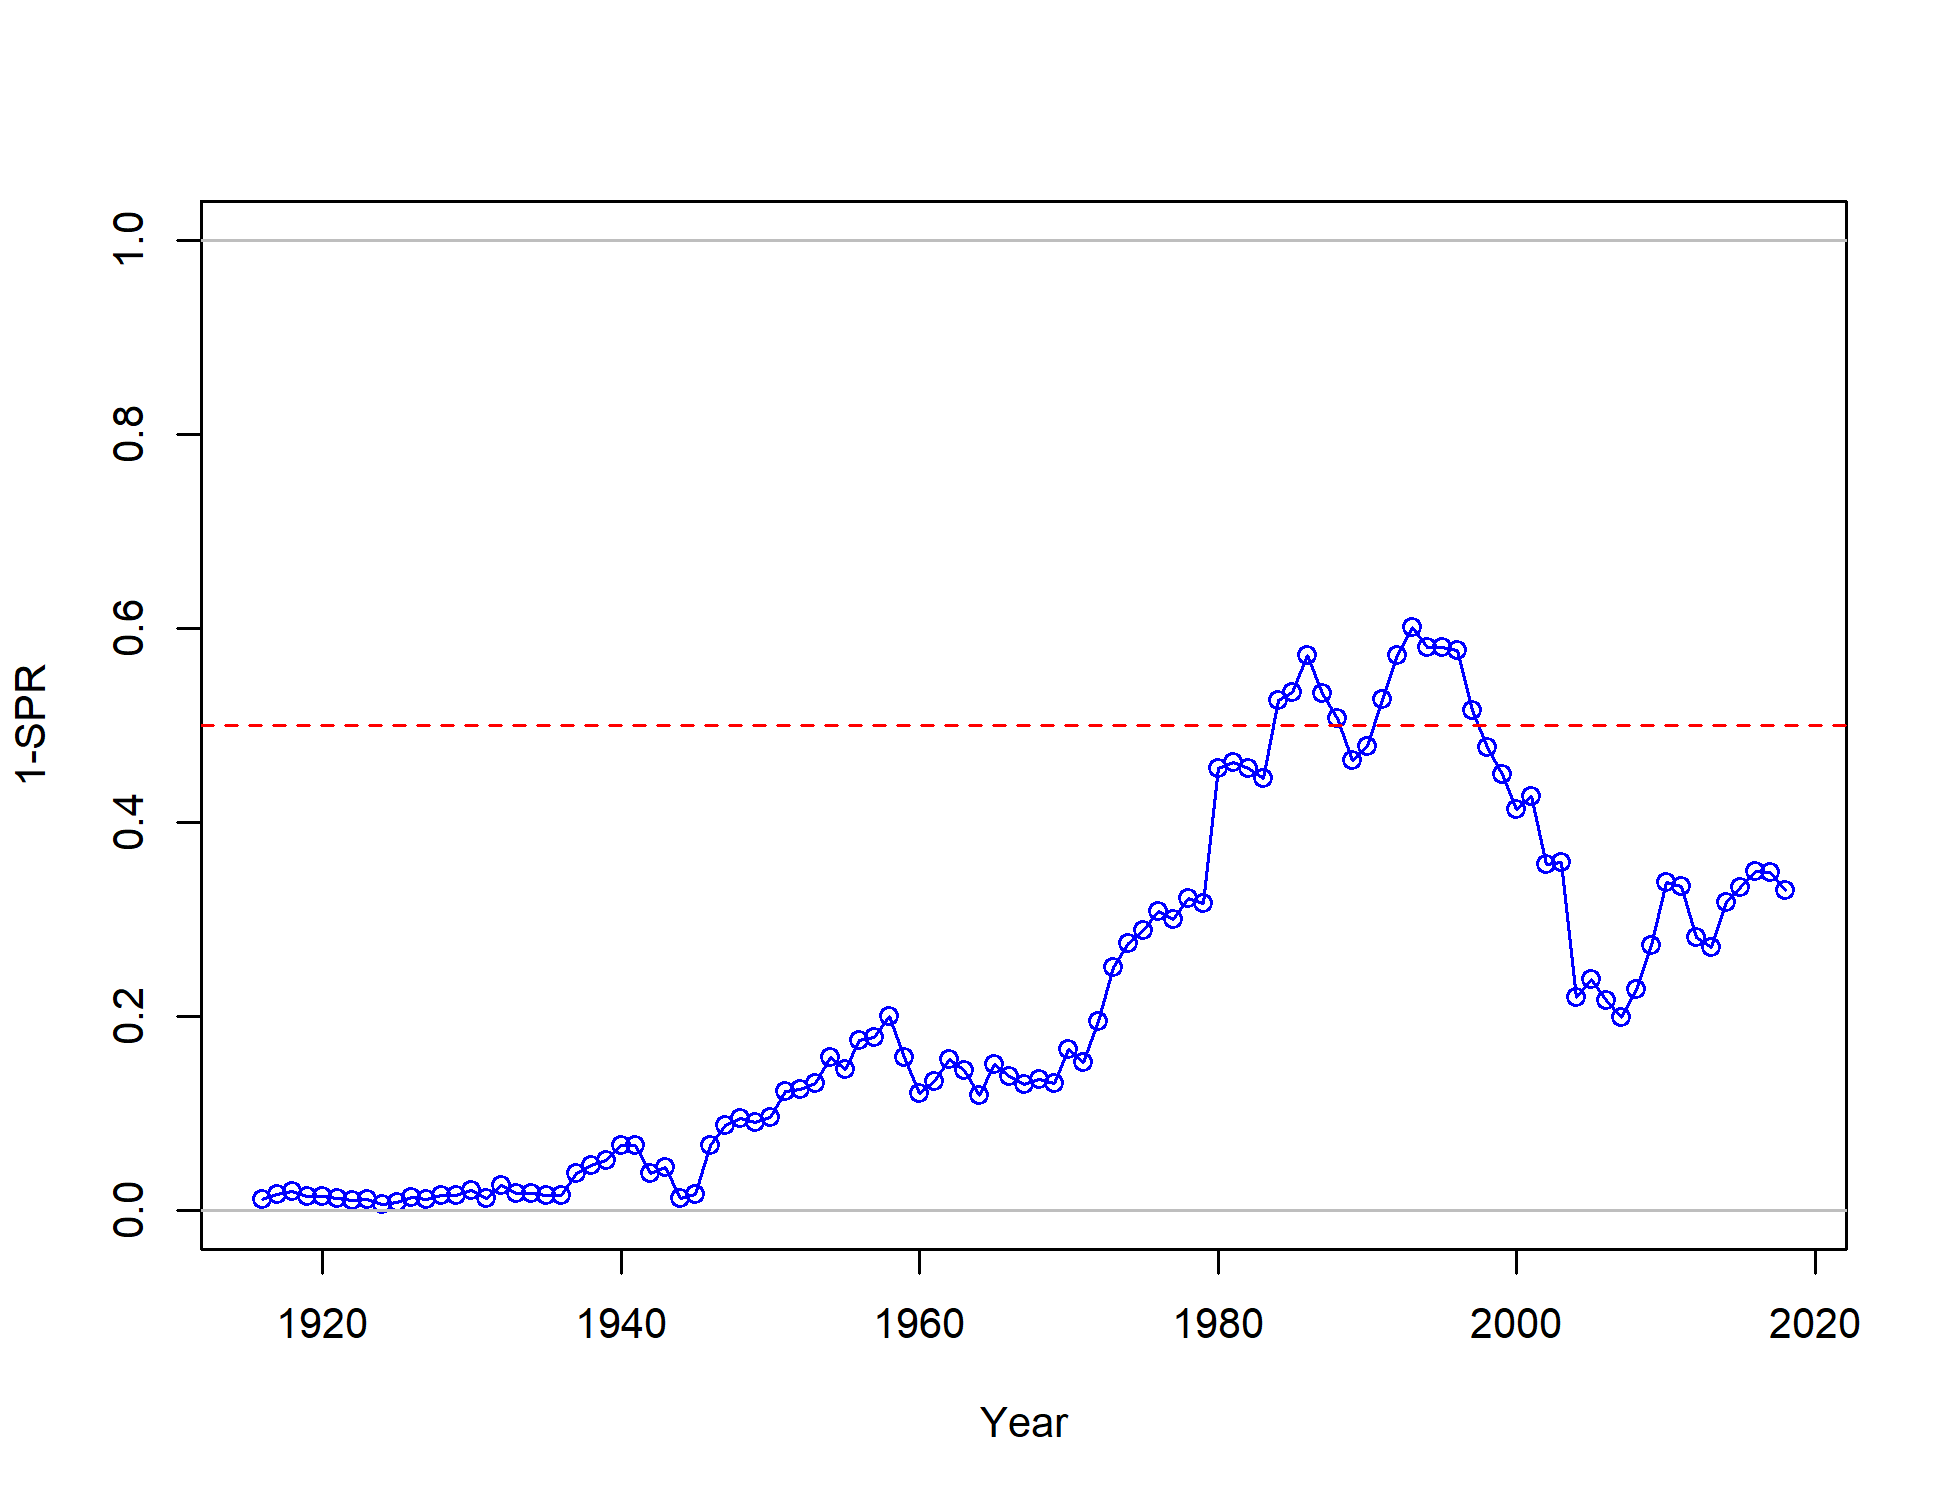
\includegraphics{r4ss/plots_mod1/SPR2_minusSPRseries.png}
\caption{Estimated spawning potential ratio (SPR) for the base-case
model. One minus SPR is plotted so that higher exploitation rates occur
on the upper portion of the y-axis. The management target is plotted as
a red horizontal line and values above this reflect harvests in excess
of the overfishing proxy based on the SPR\textsubscript{50\%} harvest
rate. The last year in the time series is 2018. \label{fig:SPR_all}}
\end{figure}

\FloatBarrier

\subsection*{Ecosystem Considerations}\label{ecosystem-considerations}
\addcontentsline{toc}{subsection}{Ecosystem Considerations}

In this assessment, ecosystem considerations were not explicitly
included in the analysis.\\
This is primarily due to a lack of relevant data and results of analyses
(conducted elsewhere) that could contribute ecosystem-related
quantitative information for the assessment.

\subsection*{Reference Points}\label{reference-points}
\addcontentsline{toc}{subsection}{Reference Points}

This stock assessment estimates that GBY rockfish in the model is above
the biomass target (\(SB_{40\%}\)), and well above the minimum stock
size threshold (\(SB_{25\%}\)). The estimated relative depletion level
for the base model in 2019 is 45.1\% (95\% asymptotic interval: \(\pm\)
28.9\%-61.3\%, corresponding to an unfished spawning biomass of 599.431
million eggs (95\% asymptotic interval: 397.31-801.55 million eggs) of
spawning biomass in the base model (Table \ref{tab:Ref_pts_mod1}).
Unfished age 1+ biomass was estimated to be 1,969 mt in the base case
model. The target spawning biomass (\(SB_{40\%}\)) is 532 million eggs,
which corresponds with an equilibrium yield of 145 mt. Equilibrium yield
at the proxy \(F_{MSY}\) harvest rate corresponding to \(SPR_{50\%}\) is
136 mt (Figure \ref{fig:Yield_all}).

\FloatBarrier

\begin{table}[ht]
\centering
\caption{Summary of reference 
                                      points and management quantities for the 
                                      base case model.} 
\label{tab:Ref_pts_mod1}
\begin{tabular}{>{\raggedright}p{4.1in}>{\raggedleft}p{.62in}>{\raggedleft}p{.62in}>{\raggedleft}p{.62in}}
  \hline
\textbf{Quantity} & \textbf{Estimate} & \textbf{Low 2.5\%  limit} & \textbf{High 2.5\%  limit} \\ 
  \hline
Unfished spawning output (million eggs) & 1,329 & 1,030 & 1,629 \\ 
  Unfished age 1+ biomass (mt) & 1,969 & 1,642 & 2,296 \\ 
  Unfished recruitment ($R_{0}$) & 3,749 & 1,561 & 5,937 \\ 
  Spawning output(2018 million eggs) & 599 & 389 & 809 \\ 
  Depletion (2018) & 0.451 & 0.34 & 0.561 \\ 
  \textbf{$\text{Reference points based on } \mathbf{SB_{40\%}}$} &  &  &  \\ 
  Proxy spawning output ($B_{40\%}$) & 532 & 456 & 607 \\ 
  SPR resulting in $B_{40\%}$ ($SPR_{B40\%}$) & 0.458 & 0.458 & 0.458 \\ 
  Exploitation rate resulting in $B_{40\%}$ & 0.139 & 0.107 & 0.171 \\ 
  Yield with $SPR_{B40\%}$ at $B_{40\%}$ (mt) & 145 & 105 & 184 \\ 
  \textbf{\textit{Reference points based on SPR proxy for MSY}} &  &  &  \\ 
  Spawning output & 593 & 509 & 677 \\ 
  $SPR_{proxy}$ & 0.5 &  &  \\ 
  Exploitation rate corresponding to $SPR_{proxy}$ & 0.121 & 0.093 & 0.15 \\ 
  Yield with $SPR_{proxy}$ at $SB_{SPR}$ (mt) & 136 & 99 & 173 \\ 
  \textbf{\textit{Reference points based on estimated MSY values}} &  &  &  \\ 
  Spawning output at $MSY$ ($SB_{MSY}$) & 297 & 248 & 346 \\ 
  $SPR_{MSY}$ & 0.299 & 0.288 & 0.31 \\ 
  Exploitation rate at $MSY$ & 0.234 & 0.171 & 0.296 \\ 
  Dead Catch $MSY$ (mt) & 165 & 117 & 212 \\ 
  Retained Catch $MSY$ (mt) & 165 & 117 & 212 \\ 
   \hline
\end{tabular}
\end{table}

\FloatBarrier

\subsection*{Management Performance}\label{management-performance}
\addcontentsline{toc}{subsection}{Management Performance}

Table \ref{tab:mnmgt_perform}

\begin{table}[ht]
\centering
\caption{Recent trend in total catch and commercial 
                              landings (mt) relative to the management guidelines. 
                              Estimated total catch reflect the commercial landings 
                              plus the model estimated discarded biomass.} 
\label{tab:mnmgt_perform}
\scalebox{0.9}{
\begin{tabular}{>{\raggedleft}p{1in}>{\centering}p{1in}>{\centering}p{1in}>{\centering}p{1in}>{\centering}p{1in}}
  \hline
Year & OFL (mt; ABC prior to 2011) & ABC (mt) & ACL (mt; OY prior to 2011) & Estimated total catch (mt) \\ 
  \hline
\textbf{2007} & - & - & - & - \\ 
  \textbf{2008} & - & - & - & - \\ 
  \textbf{2009} & - & - & - & - \\ 
  \textbf{2010} & - & - & - & - \\ 
  \textbf{2011} & - & - & - & - \\ 
  \textbf{2012} & - & - & - & - \\ 
  \textbf{2013} & - & - & - & - \\ 
  \textbf{2014} & - & - & - & - \\ 
  \textbf{2015} & - & - & - & - \\ 
  \textbf{2016} & - & - & - & - \\ 
  \textbf{2017} & - & - & - & - \\ 
  \textbf{2018} & - & - & - & - \\ 
   \hline
\end{tabular}
}
\end{table}

\subsection*{Unresolved Problems and Major
Uncertainties}\label{unresolved-problems-and-major-uncertainties}
\addcontentsline{toc}{subsection}{Unresolved Problems and Major
Uncertainties}

\FloatBarrier

\subsection*{Decision Table}\label{decision-table}
\addcontentsline{toc}{subsection}{Decision Table}

\begin{table}[ht]
\centering
\caption{Projections of potential OFL (mt) for 
                                        each model, using the base model forecast.} 
\label{tab:OFL_projection}
\begin{tabular}{lr}
  \hline
Year & OFL \\ 
  \hline
2019 & 145.83 \\ 
   \hline
\end{tabular}
\end{table}\begin{table}[ht]
\centering
\caption{Summary of 10-year 
                                             projections beginning in 2020 
                                             for alternate states of nature based on 
                                             an axis of uncertainty for the model.  Columns range over low, mid, and high
                                             states of nature, and rows range over different 
                                             assumptions of catch levels. An entry of "--" 
                                             indicates that the stock is driven to very low 
                                             abundance under the particular scenario.} 
\label{tab:Decision_table_mod1}
\scalebox{0.85}{
\begin{tabular}{l|cc|>{\centering}p{.7in}c|>{\centering}p{.7in}c|>{\centering}p{.7in}c}
   \multicolumn{3}{c}{}  &  \multicolumn{2}{c}{} 
                               & \multicolumn{2}{c}{\textbf{States of nature}} 
                               & \multicolumn{2}{c}{} \\
  \multicolumn{3}{c}{}  &  \multicolumn{2}{c}{Low M 0.05} 
                               & \multicolumn{2}{c}{Base M 0.07} 
                               &  \multicolumn{2}{c}{High M 0.09} \\
 \hline
 & Year & Catch & Spawning Output & Depletion & Spawning Output & Depletion & Spawning Output & Depletion \\ 
  \hline
 & 2019 & - & - & - & - & - & - & - \\ 
   & 2020 & - & - & - & - & - & - & - \\ 
   & 2021 & - & - & - & - & - & - & - \\ 
  40-10 Rule,  & 2022 & - & - & - & - & - & - & - \\ 
  Low M & 2023 & - & - & - & - & - & - & - \\ 
   & 2024 & - & - & - & - & - & - & - \\ 
   & 2025 & - & - & - & - & - & - & - \\ 
   & 2026 & - & - & - & - & - & - & - \\ 
   & 2027 & - & - & - & - & - & - & - \\ 
   & 2028 & - & - & - & - & - & - & - \\ 
   \hline
 & 2019 & - & - & - & - & - & - & - \\ 
   & 2020 & - & - & - & - & - & - & - \\ 
   & 2021 & - & - & - & - & - & - & - \\ 
  40-10 Rule & 2022 & - & - & - & - & - & - & - \\ 
   & 2023 & - & - & - & - & - & - & - \\ 
   & 2024 & - & - & - & - & - & - & - \\ 
   & 2025 & - & - & - & - & - & - & - \\ 
   & 2026 & - & - & - & - & - & - & - \\ 
   & 2027 & - & - & - & - & - & - & - \\ 
   & 2028 & - & - & - & - & - & - & - \\ 
   \hline
 & 2019 & - & - & - & - & - & - & - \\ 
   & 2020 & - & - & - & - & - & - & - \\ 
   & 2021 & - & - & - & - & - & - & - \\ 
  40-10 Rule, & 2022 & - & - & - & - & - & - & - \\ 
  High M & 2023 & - & - & - & - & - & - & - \\ 
   & 2024 & - & - & - & - & - & - & - \\ 
   & 2025 & - & - & - & - & - & - & - \\ 
   & 2026 & - & - & - & - & - & - & - \\ 
   & 2027 & - & - & - & - & - & - & - \\ 
   & 2028 & - & - & - & - & - & - & - \\ 
   \hline
 & 2019 & - & - & - & - & - & - & - \\ 
   & 2020 & - & - & - & - & - & - & - \\ 
   & 2021 & - & - & - & - & - & - & - \\ 
  Average & 2022 & - & - & - & - & - & - & - \\ 
  Catch & 2023 & - & - & - & - & - & - & - \\ 
   & 2024 & - & - & - & - & - & - & - \\ 
   & 2025 & - & - & - & - & - & - & - \\ 
   & 2026 & - & - & - & - & - & - & - \\ 
   & 2027 & - & - & - & - & - & - & - \\ 
   & 2028 & - & - & - & - & - & - & - \\ 
   \hline
\end{tabular}
}
\end{table}

\begin{sidewaystable}[ht]
\centering
\caption{Base case results summary.} 
\label{tab:base_summary}
\scalebox{0.6}{
\begin{tabular}{r>{\centering}p{1.1in}>{\centering}p{1.1in}>{\centering}p{1.1in}>{\centering}p{1.1in}>{\centering}p{1.1in}>{\centering}p{1.1in}>{\centering}p{1.1in}>{\centering}p{1.1in}>{\centering}p{1.1in}>{\centering}p{1.1in}}
  \hline
Quantity & 2010 & 2011 & 2012 & 2013 & 2014 & 2015 & 2016 & 2017 & 2018 & 2019 \\ 
  \hline
Landings (mt) &  &  &  &  &  &  &  &  &  &  \\ 
  Total Est. Catch (mt) &  &  &  &  &  &  &  &  &  &  \\ 
  OFL (mt) &  &  &  &  &  &  &  &  &  &  \\ 
  ACL (mt) &  &  &  &  &  &  &  &  &  &  \\ 
   \hline
(1-$SPR$)(1-$SPR_{50\%}$) & 0.82 & 0.81 & 0.71 & 0.67 & 0.78 & 0.81 & 0.85 & 0.85 & 0.81 &  \\ 
   \hline
Exploitation rate & 0.11 & 0.11 & 0.08 & 0.07 & 0.09 & 0.10 & 0.10 & 0.10 & 0.08 &  \\ 
  Age 1+ biomass (mt) & 1391.63 & 1332.20 & 1246.97 & 1184.00 & 1156.13 & 1140.65 & 1116.13 & 1101.05 & 1097.89 & 1118.10 \\ 
   \hline
Spawning Output & 864.6 & 795.9 & 741.2 & 711.8 & 691.1 & 661.0 & 634.7 & 612.7 & 599.1 & 599.4 \\ 
  ~95\% CI & (604.3-1124.85) & (549.68-1042.04) & (507.57-974.88) & (487.79-935.76) & (474.44-907.77) & (449.78-872.25) & (425.9-843.51) & (404.15-821.3) & (389.03-809.08) & (397.31-801.55) \\ 
   \hline
Depletion & 0.7 & 0.6 & 0.6 & 0.5 & 0.5 & 0.5 & 0.5 & 0.5 & 0.5 & 0.5 \\ 
  ~95\% CI & (0.515-0.786) & (0.471-0.726) & (0.437-0.678) & (0.421-0.65) & (0.41-0.63) & (0.39-0.604) & (0.371-0.584) & (0.353-0.569) & (0.34-0.561) & (0.289-0.613) \\ 
   \hline
Recruits & 3218.83 & 2746.99 & 2631.66 & 2767.28 & 3916.77 & 5510.34 & 4079.14 & 3360.32 & 2968.86 & 3352.25 \\ 
  ~95\% CI & (1410.42 - 7345.97) & (1180.57 - 6391.77) & (1126.64 - 6147.16) & (1179.6 - 6491.88) & (1632.26 - 9398.66) & (2305.44 - 13170.55) & (1645.01 - 10115.07) & (1372 - 8230.16) & (1262.36 - 6982.25) & (1373.02 - 8184.58) \\ 
   \hline
\end{tabular}
}
\end{sidewaystable}

\begin{figure}
\centering
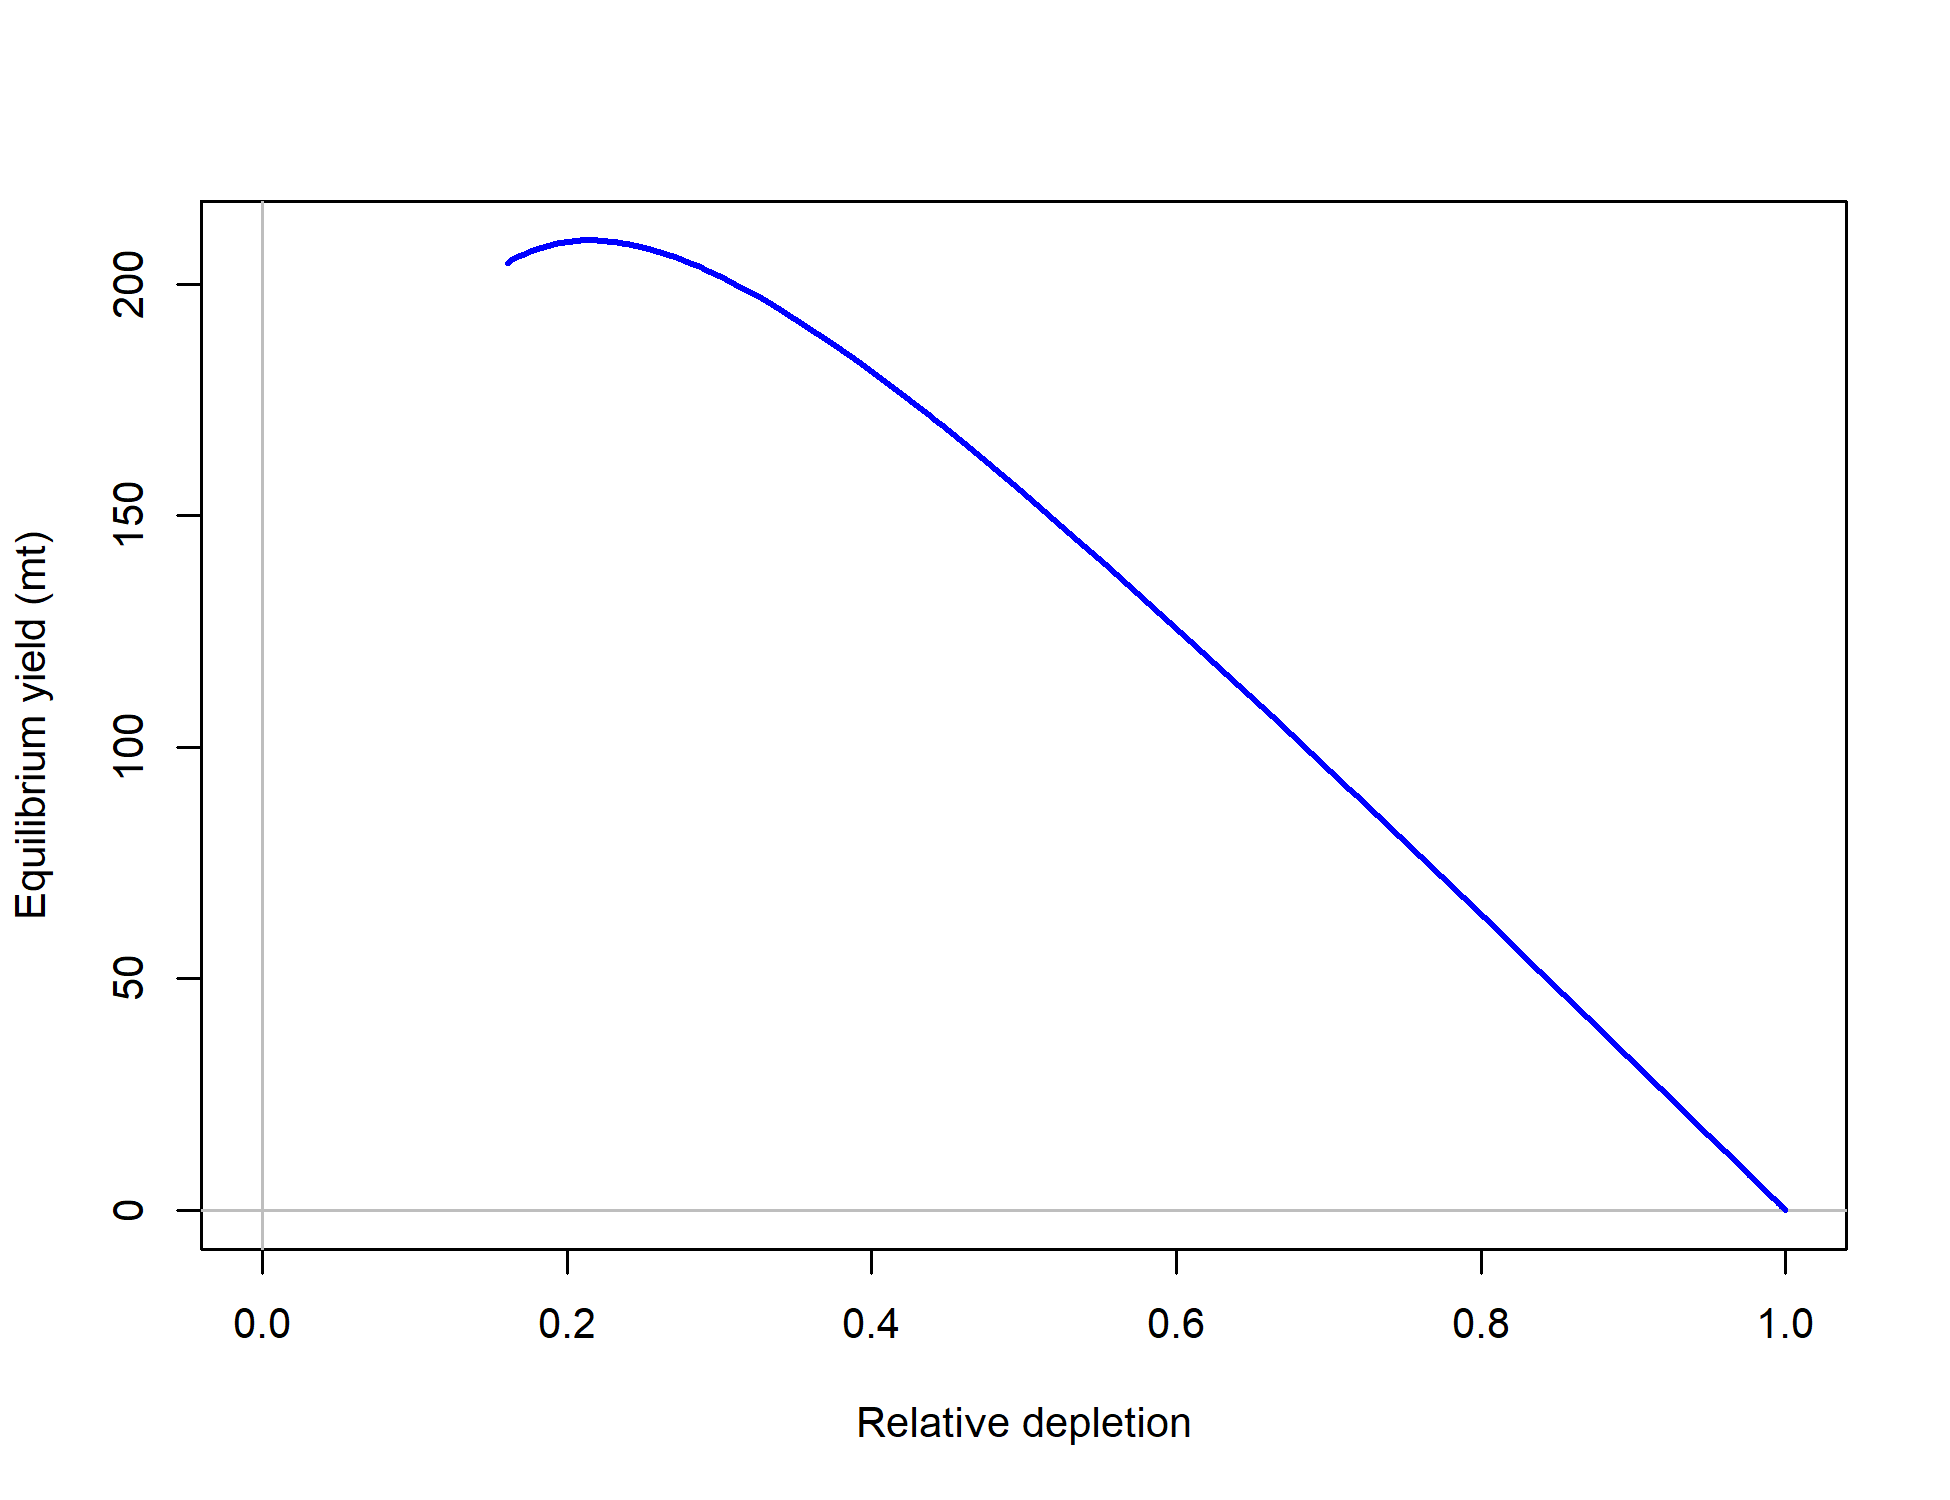
\includegraphics{r4ss/plots_mod1/yield1_yield_curve.png}
\caption{Equilibrium yield curve for the base case model. Values are
based on the 2018 fishery selectivity and with steepness fixed at 0.718.
\label{fig:Yield_all}}
\end{figure}

\FloatBarrier

\newpage

\subsection*{Research and Data Needs}\label{research-and-data-needs}
\addcontentsline{toc}{subsection}{Research and Data Needs}

We recommend the following research be conducted before the next
assessment:

\begin{enumerate}

\item \textbf{xxxx}: 

\item \textbf{xxxx}:

\item \textbf{xxxx}:

\item \textbf{xxxx}:

\item \textbf{xxxx}:

\end{enumerate}

\FloatBarrier

\newpage

\renewcommand{\thefigure}{\arabic{figure}}
\renewcommand{\thetable}{\arabic{table}}

\setcounter{figure}{0} \setcounter{table}{0}

\newpage

\color{black}

\section*{References}\label{references}
\addcontentsline{toc}{section}{References}

\renewcommand{\thepage}{}

\end{document}
